\documentclass[twocolumn]{article}

%%%%%%%%%%%%%%%%%%%%%%%%%%%%%%%%%%%%%%%%%%%%%%%
%% Comment / uncomment for one or two column(s) fomat
%\documentclass{article}

\usepackage[modulo,switch]{lineno}
\modulolinenumbers[1]
%%%%%%%%%%%%%%%%%%%%%%%%%%%%%%%%%%%%%%%%%%%%%%%
%% Comment / uncomment for showing line numbers
\linenumbers

\usepackage[latin9]{inputenc}
\usepackage{amsmath}
\usepackage{amssymb}
\usepackage{graphicx}

\makeatletter\@ifundefined{date}{}{\date{}}
\makeatother

\markright{\hfill Gontier {\em et al.}, p.\ }
\pagestyle{myheadings}

\paperheight297mm \paperwidth210mm
\textwidth170mm  \textheight245mm  \oddsidemargin 20mm
\evensidemargin\oddsidemargin \hoffset-22.4mm \voffset-28.4mm
\topmargin0pt \headheight20mm \headsep4mm \topskip0mm
\footskip17.5mm \columnsep7mm \arraycolsep2pt \parindent10pt
\renewcommand{\abstractname}{Summary}


\usepackage[english]{babel}
\usepackage[T1]{fontenc}

\usepackage{amsmath}
\usepackage{amsfonts}
\usepackage{amssymb}
\usepackage{fancyhdr}
\usepackage[hidelinks]{hyperref}
\usepackage{graphicx}
\usepackage{epstopdf}
\usepackage{pdflscape}
\usepackage{multirow}
\usepackage{subcaption}
\usepackage{bbm}
\usepackage{color}
\DeclareMathOperator*{\argmax}{arg\,max}
\newcommand{\ml}[1]{\textcolor{red}{ML : #1}}
\begin{document}
\author{F\'elix Gontier $^1$, Catherine Lavandier $^2$, Pierre Aumond $^{2, 3}$\\Mathieu Lagrange $^1$, Jean-Francois Petiot $^1$}
\date{
$^1$ LS2N, UMR CNRS 6004, Ecole Centrale de Nantes, F-44321, France\\
$^2$ ETIS, UMR CNRS 8051, University of Paris Seine, University of Cergy-Pontoise, ENSEA, CNRS, F-95000, France\\
$^3$ IFSTTAR, CEREMA, UMRAE, F-44344, Bouguenais, France
}
\title{Estimation of the perceived time of presence of sources in urban acoustic environments using deep learning techniques}
\maketitle


\begin{abstract}

The impact of urban sound on human beings has often been studied from a negative point of view (sound pollution). In the two last decades, the interest of studying its positive impact has been revealed with the soundscape approach (resourcing spaces). The literature shows that the recognition of sources plays a great role in the way humans are affected by sound environments. There is thus a need for characterizing urban acoustic environments not only with sound pressure measurements but also with source-specific attributes such as their perceived time of presence.

This paper demonstrates, on a controlled dataset, that machine learning techniques based on state of the art neural architectures can predict the perceived time of presence of several sound sources at a sufficient accuracy. To validate this assertion, a corpus of simulated sound scenes is first designed. Perceptual attributes corresponding to those stimuli are gathered through a listening experiment. The availability of the contributions of the individual sound sources within the simulated sound scenes allows the computation of a physical indicator approximating the perceived time of presence of sources, then used for the training and validation of the proposed estimation procedure. The resulting model predicts the time of presence with excellent performance, which translates to the estimation of pleasantness in urban sound environments at a sufficient degree of precision.

PACS numbers: 43.66.Lj (Perceptual effects of sound), 43.60.-c (Acoustic signal processing)
\end{abstract}


\section{Introduction}
\label{sec:intro}

%In urban areas, the decrease of quality of sound environments resulting from urbanization is a major cause of annoyance, and has been identified as an important health factor. Consequently, the 2002/49/EC European directive~\cite{ec2002} requires the development of noise maps in large cities. These maps aim at providing useful tools for noise reduction planning purposes. In this context, the soundscape approach defined in the ISO 12913-1~\cite{iso2014} norm as the "acoustic environment as perceived or experienced and/or understood by people, in context" provides a shift from the noise-only paradigm by considering the possible positive influence of some the sound environment's components.

Leveraging the advent of the Internet of Things (IoT) and the availability of low-cost sensor networks~\cite{ardouin2018, mydlarz2017} could allow us to characterize the sound environment in a way that is closer to the perception of city dwellers~\cite{iso2014}. This requires the identification of its composition in terms of sources of interest from acoustic measurements at a reasonable cost. Most monitoring applications mainly rely on the measurement of sound levels on time scales from 1s to several hours~\cite{can2008, brocolini2013}, which offers limited information regarding the content of the sound environment. Conversely, sound environment recognition and event detection applications operate on spectral representations of recorded audio on much finer time scales, in tens of milliseconds~\cite{lunden2016, aucouturier2007, cakir2015}. While using such information-rich representations of the signal also allows the computation of commonly used monitoring acoustical indicators, it may not be desirable in long-term monitoring applications where analysis is performed offline. Indeed, it requires large transmission bandwidth and storage capabilities, and raises privacy concerns if intelligible speech can be retrieved. Some monitoring applications~\cite{aumond2017, torija2013, nilsson2007} use third octave sound level fast (125ms) measurements to underline relevant spectral information. This representation is easier to store in the long term and reduces privacy concerns~\cite{gontier2017}. In~\cite{aumond2017}, the authors successfully linked acoustical indicators derived from third octave sound levels to the perceived activity of specific sound sources in recordings of polyphonic sound scenes. Though the discriminative properties of the proposed indicators are limited and the underlying methodology cannot be easily extended to larger sound source taxonomies, it demonstrates that the information content of third octave spectra is sufficient to identify sound sources.

The characterization of urban soundscapes through standardized perceptual descriptors has been extensively studied~\cite{viollon2000, axelsson2010, cain2013, jeon2018, aletta2016}. A two-dimensional soundscape model of perceived quality emerges where one dimension corresponds to the pleasantness of the soundscape, and the orthogonal one corresponds to its enventfulness~\cite{axelsson2010, aumond2017, delaitre2014}. Three major source types are found to contribute to these dimensions in urban contexts: technological, human and natural sources~\cite{nilsson2007, axelsson2010}, though the exact taxonomy of sources used differs across studies~\cite{guastavino2007, gygi2007, brown2011}. Furthermore, traffic noise, human voices and birds calls can respectively be used as a proxy of these source types~\cite{lavandier2006, ricciardi2014, aumond2017}. In existing models, source activity can be quantified by the dominance~\cite{hong2017, axelsson2010} or the time of presence~\cite{ricciardi2014}. The perceived time of presence has the advantage of considering all simultaneously active sources, and its identification from acoustic monitoring measurements would provide more complete information on the content of polyphonic urban environments~\cite{lavandier2016}.

In this paper, we do so by developing new indicators relying on source recognition models based on deep learning techniques, which has demonstrated state-of-the-art performance in many tasks studied in the machine listening community~\cite{mesaros2017}. In the context of urban sound environments, deep learning has successfully been applied to sound event detection~\cite{foggia2015, mcfee2018, adavanne2017} and sound scene classification~\cite{valenti2016, salamon2017-2}. Several architectures may be used to this aim, the most common of which are convolutional and recurrent neural networks~\cite{mesaros2019}. Learning-based approaches mainly process spectral representations of the audio, such as Mel spectrograms or Mel frequency cepstrum coefficients~\cite{barchiesi2015}. Large amounts of data with task-specific annotations are required for deep learning architectures to learn to extract relevant information from recordings~\cite{salamon2014, mesaros2017, gemmeke2017}. To the best of our knowledge such databases do not currently exist in the literature in the case of source recognition with labels consisting of perceived source activity. It is possible to manually annotate each recording in the corpus. However, this process would be time-consuming, and must be repeated to extend the taxonomy of relevant sound sources. As an alternative, we consider the use of simulated corpora~\cite{lafay2016, salamon2017}, of which the generation procedure provides complete knowledge about the composition of sound scenes. By using a simple indicator computed on this information-rich data to approximate the source-specific perceived time of presence labels, the excerpts composing large corpora may be automatically annotated without the need for additional subjective inputs. Thanks to this data generation procedure, we are able to validate the proposed approach.

More precisely, the contributions of this paper are three-fold:
\begin{enumerate}
  \item Provide a corpus of simulated scenes for which relevant acoustic properties are well controlled and perceptual judgements are available\footnote{Corpus available at \url{https://zenodo.org/record/3248734\#.XQjC4v7gqUk}}.
  \item Propose numerical means\footnote{Open source code is available at \url{https://github.com/felixgontier/soundSourcePresenceEstimation}.} for predicting the perceived time of presence of sound sources from raw acoustic data using deep learning approaches, with a larger corpus of simulated scenes\footnote{Corpus available at \url{https://zenodo.org/record/3248703\#.XQjDVv7gqUk}}.
  \item Demonstrate that the proposed method can be applied to the prediction of a perceptual descriptor of soundscapes to a sufficient degree of accuracy through a comparative study with state of the art approaches.
\end{enumerate}

The procedure for simulating sound scenes corpora is presented in Section~\ref{sec:data} with the outcomes of the listening test conducted to justify the relevance of the sound scenes corpora in the context of a study on perceived quality. A large corpus is constructed and used to train and evaluate a deep learning architecture that performs multi-label sound source recognition at relevant time scales, as presented in Section~\ref{sec:pred}. The application of the resulting time of presence to the prediction of pleasantness in urban environments is then presented in Section~\ref{sec:app}.%The, in comparison to existing models from perceptual and physical indicators.



\section{Corpus}
\label{sec:data}


\subsection{Generation procedure}
\label{sec:data_corp}

Considering machine learning techniques to detect the presence of sources requires the availability of annotated data. Thus, in order to train deep learning architectures for source recognition, a large corpus is constructed. This corpus is composed of sound scenes simulated using the \textit{simScene} software, an open source software library in Matlab that allows the simulation of sound scenes as the additive composition of sound sources, using a database of recordings associated to isolated occurences of these sources\footnote{\url{https://bitbucket.org/mlagrange/simscene}}. Here we choose to restrict the taxonomy of active sources to \textit{traffic}, \textit{human voices} and \textit{birds}, as these sources are found to be the most influent on soundscape quality~\cite{lavandier2006}. The corresponding database of isolated is constructed from excerpts of the LibriSpeech~\cite{panayotov2015} corpus for voices and Freesound\footnote{\url{https://freesound.org}} contributions for remaining sources. \textit{simScene} generates original scenarios using the following information:

\begin{itemize}
\item The probability of appearance of a given source in the scene, for which events and backgrounds are considered separately,
\item Event-to-background ratios (EBR) in dB for all events and backgrounds compared to a main background source, drawn from gaussian distributions,
\item The inter-onset of event occurrences in seconds, also drawn from gaussian distributions.
\end{itemize}

Newly generated scenarios should cover most real-life situations while remaining perceptually plausible. To do so, a corpus of 74 recordings obtained in~\cite{aumond2017} is taken as reference. The recordings include 19 locations in the 13th district of Paris, France. A classification of these scenes is proposed in~\cite{gloaguen2017} in terms of ambiance: \textit{park}, \textit{quiet street}, \textit{noisy street} and \textit{very noisy street}. The statistics on background and event properties needed for \textit{simScene} generation are extracted conditionally on the ambiance from annotations of the corpus presented in~\cite{gloaguen2017}, which include:

\begin{itemize}
\item Background sources that are present throughout the whole scene, and their respective sound level considered constant,
\item Sound events characterized for each occurrence by their source type, onset-offset and event-to-background ratio (EBR) in dB.
\end{itemize}

Adjustments are made on the variance of the considered properties to better cover possible scenarios. Furthermore, since voice events in the isolated source database consist mostly of read English recordings, voice event mean EBR are reduced to improve realism. An additional \textit{square} ambiance is added with properties derived empirically from available data. Diverse new scenarios are then generated by sampling the background and event properties distributions and used with samples randomly selected from the database of isolated occurrences to simulate sound scenes. At the end of the simulation process the sound level of each sound scene is randomly sampled and conditioned to the ambiance according to typical sound levels in urban context.

The simulated deep learning corpus is composed of two subsets:
\begin{itemize}
\item The development set, made of 400 scenes of 45~s each (total duration 5 hours), which is used during the training process,
\item The evaluation set, made of 200 scenes of 45~s each (total of 2.5 hours), which is used to compute the performance of the trained model and its generalization capabilities.
\end{itemize}

The generation procedure is the same for both datasets. Though, it is important in deep learning applications to ensure a complete independance of the training and test set. To do so, the isolated samples database is split in the same proportions as the two datasets: two-thirds for the development set and the remaining one-third for the evaluation set. As a result, while the generation process is the same for both corpora, the scenarios and audio samples are different.

\subsection{Perceptual experiment}
\label{sec:data_exp}

An experiment in the form a listening test is conducted in order to validate the perceptual correspondence of the proposed corpus with urban sound scene recordings, as well as obtain subjective annotations for the design and evaluation of a time of presence estimation model.

Given the aim of this test, a separate corpus is constructed. First, 200 simulated scenes of 45s each with diverse new scenarios are generated with the procedure described in Section~\ref{sec:data_corp}, though with a separate database of isolated source occurences. These scenes are equally distributed among the five considered ambiances (resp. \textit{park}, \textit{quiet street}, \textit{noisy street}, \textit{very noisy street} and \textit{square}). For each scene the perceived time of presence for the traffic, voice and bird sources is estimated using the indicators proposed in~\cite{gontier2018}. Ideally, sound scenes should cover the resulting 3-dimensional space in a homogeneous way. To do so, the 75 scenes that maximize the minimum pairwise distance in the 3-dimensional space are selected. The distribution of selected extracts is shown in Figure~\ref{fig:tvb_pres}. Playback sound levels are realistically drawn as described in Section~\ref{sec:data_corp} and range from 46.6~dB SPL to 77.1~dB SPL over the 75 sound scenes.

\begin{figure*}[th]
    \centering
     \begin{subfigure}[t]{0.33\textwidth}
        \centering
        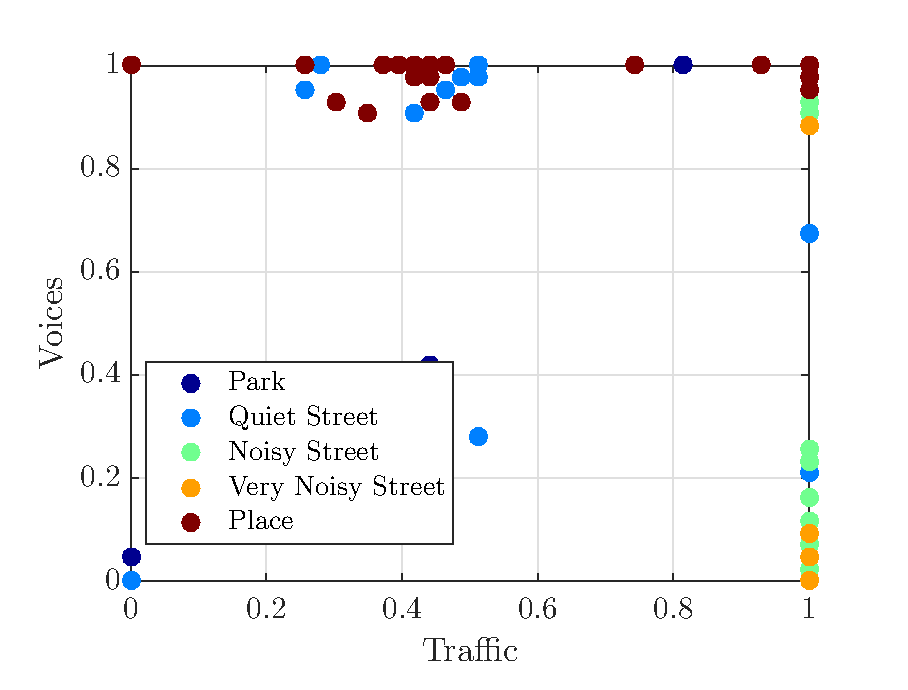
\includegraphics[width=\textwidth]{figures/tv_pres.eps}
    \end{subfigure}%
    \begin{subfigure}[t]{0.33\textwidth}
        \centering
        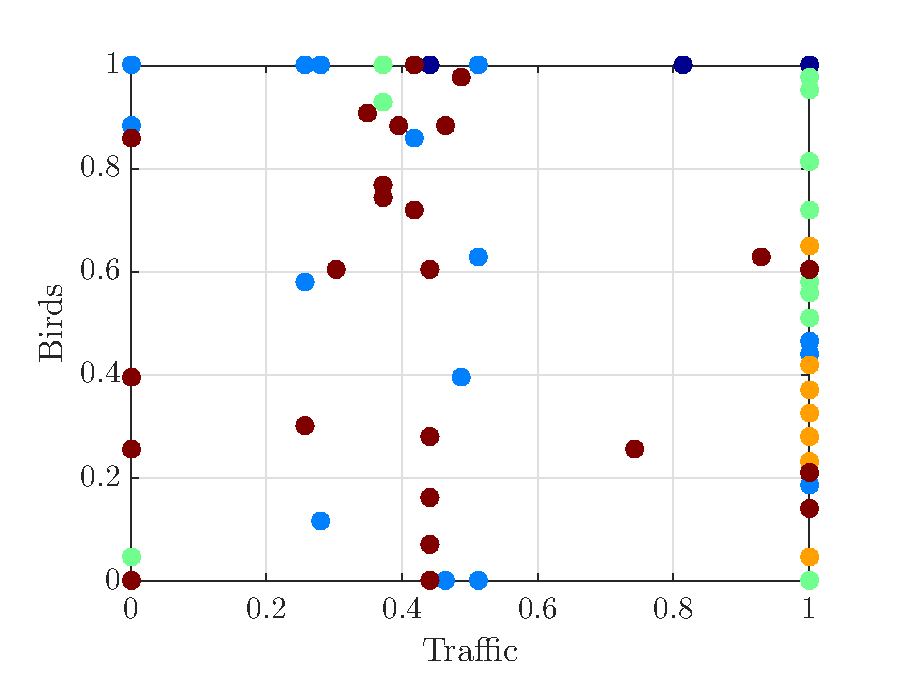
\includegraphics[width=\textwidth]{figures/tb_pres.eps}
    \end{subfigure}
    \begin{subfigure}[t]{0.33\textwidth}
        \centering
        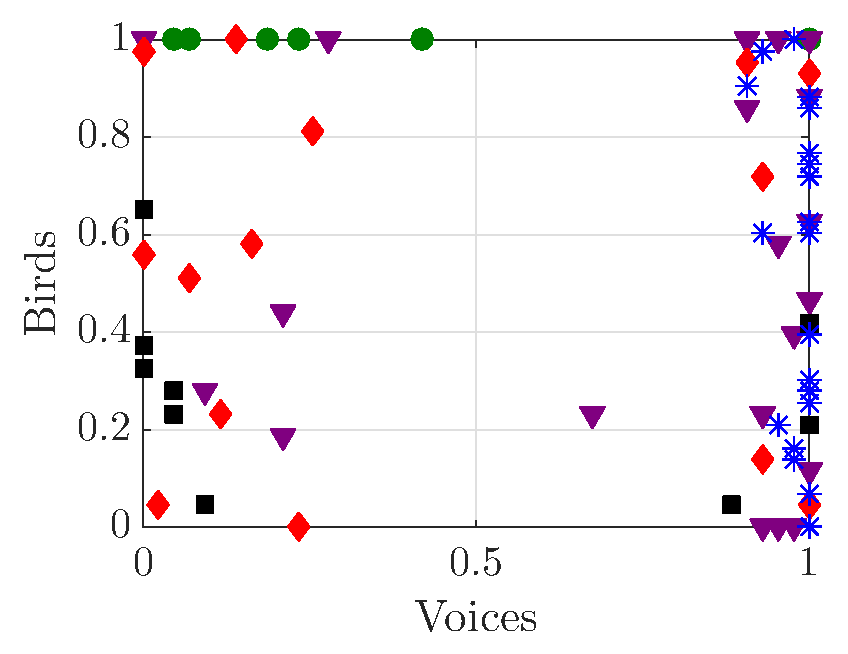
\includegraphics[width=\textwidth]{figures/vb_pres.eps}
    \end{subfigure}
    \caption{Physical estimations~\cite{gontier2018} of the perceived time of presence of traffic, voices and birds sources for the corpus of simulated scenes with automatically generated scenarios.}\label{fig:tvb_pres}
\end{figure*}

In order to validate the generation procedure of new scenarios, the listening test corpus is extended with replications of recorded sound scenes. Reference recordings are obtained from one of the four soundwalks performed in~\cite{aumond2017}, including 19 locations (noted P1-19) with diverse environments. For each of the 19 corresponding recordings, 45 seconds of audio in a single channel are extracted. The 45~s segments are selected to represent the properties of their respective ambiances in terms of source composition, without single events overwhelming their overall perception. The annotations obtained in~\cite{gloaguen2017} in terms of background and event information are then used to replicate the sound scenes using \textit{simScene}. Furthermore, the original recordings from 6 locations (P1, P3, P4, P8, P15 and P18) are added to the experiment corpus to evaluate changes in perception yielded by the replication process, as they explore diverse real-life situations with respect to ambiance categorization. The 6 recorded and 19 replicated scenes are normalized so that their playback sound level through the restitution system is the same as measured during recording, with a range from 63.9~dB SPL to 79.4~dB SPL.

The experiment corpus thus totals 100 scenes: 6 recorded, 19 replicated scenes from the Grafic project, and 75 simulated scenes.\\


During the test, participants are asked to evaluate sound scenes in terms of 9 criteria represented by 11 point scales (0-10). These scales are presented in French and translated in this report using standard terminology. The first 5 scales relate to general properties of the scene:
\begin{itemize}
\item Pleasantness: \textit{Unpleasant - Pleasant} (\textit{D\'esagr\'eable - Agr\'eable}) - P,
\item Liveliness: \textit{Inert, amorphous - Lively, eventful} (\textit{Inerte, amorphe - Anim\'e, mouvement\'e}) - L,
\item Overall loudness: \textit{Quiet - Noisy} (\textit{Silencieux - Bruyant}) - OL,
\item Interest: \textit{Boring, uninteresting - Stimulating, interesting} (\textit{Ennuyeux, inint\'eressant - Stimulant, int\'eressant}) - I,
\item Calmness: \textit{Agitated, chaotic - Calm, peaceful} (\textit{Agit\'e, chaotique - Calme, tranquille}) - C.
\end{itemize}

These quantities are typically studied in the perceptual characterization of sound scenes~\cite{axelsson2010, aumond2017, nilsson2007}. The perceived time of presence, that is the percentage of time for which the corresponding source is heard, is selected as the activity descriptor for this study. The influence of traffic on perception is further separated into that of background and salient events. Thus, 4 additional questions are presented to the participants and evaluated on the same 11 point scales:
\begin{itemize}
\item Sound level of passing vehicles: \textit{Very low - Very high} (\textit{Tr\`es faible - Tr\`es fort}) - $L_{T, p}$,
\item Time of presence of Traffic, Voices, Birds: \textit{Never - Continuously} (\textit{Jamais - Continuellement}) - resp. $T_{T, p}$, $T_{V, p}$ and $T_{B, p}$
\end{itemize}
where $p$ denotes a perceptual evaluation.

Prior to the test, a short verbal introduction is given to the participants and the interface is introduced to ensure that the quantities are well understood. Although the corpus is comprised of 100 sound scenes, participants only evaluate 50 scenes: all listen to the 6 recorded and 19 replicated sound scenes, then to 25 of the 75 simulated with new scenarios according to a balanced incomplete block design~\cite{dagnelie2003}. The selection of simulated scenes is done so that all scenes in the sub-corpus are evaluated by the same number of participants. All participants are first presented with the most quiet then loudest of the recorded scenes (resp. P3 and P15). A random listening order is generated for each subject to control ordering effects for the remaining of the test. Participants can listen to each scene once, and have to listen to the full extract and to answer all questions before being allowed to proceed to the next scene.

The scenes are played at a given sound level as discussed in Section~\ref{sec:data_corp}, through the same computer and sound card configurations. Beyerdynamics DT-990 Pro headphones are used by all participants. The calibration of the headphone was carried out in a free field situation (pink noise through a Genelec 1031A loudspeaker in front of the head) and consisted in characterizing the relationship between voltage at the headphone terminal and the sound pressure at the entrance of a blocked ear canal. To do so, small DPA 4060 microphones have been set at the entrance of the ear canals of a human subject~\cite{moller1992}. From this information a scaling factor is applied to the sound scenes to ensure that they are heard at the desired sound level by every listener.

A total of 23 students aged from 22 to 23 years including 16 males and 7 females at Ecole Centrale de Nantes completed the test (note that with 23 subjects, the incomplete block design is not perfectly balanced). All gave consent prior to the experiment and reported normal hearing.


\subsection{Simulated corpus validation}
\label{sec:data_val}

The perceptual responses of the 6 recorded and corresponding replicated scenes are first studied. Table~\ref{tab:ogrep} shows the mean differences between assessments for pairs of scenes with equivalent scenarios. Wilcoxon signed-rank tests~\cite{wilcoxon1945} are implemented for each scene and perceptual scale to outline significant differences between assessment distributions, which are shown in bold. As the data is discretely distributed, zero differences between paired samples are included using Pratt's modification of the test~\cite{pratt1959}. On the first five scales, all mean differences are lower than 2 points on the 11-point Likert scale. Though, significant differences are outlined that can be linked to corresponding discrepancies in source-specific parameters. The highest difference (-5.22) is found for the assessment of the time of presence of traffic in the location P4. For this location, the background traffic in the recorded scene varies along time, it is louder in the first half of the scene than in the second half. Replicating this scene using simScene imposes a constant sound level for background sources. Thus, the background traffic is louder in the replicated scene than it is in the recording for about half of its duration. To a lesser extent the same issue explains the large difference (-4) in the assessed time of presence of voices in the location P3. Discrepancies on source-specific scales can also be interpreted by the choice of isolated samples, which is semi-random and based on a high-level source taxonomy. For example, no difference is made during annotation between child or adult speech, or depending on its expressiveness. Though, overall no consistent difference between the perception of recorded and replicated scenes emerges for the studied points.

\begin{table*}[t]
\centering
\caption{Mean differences of perceptual assessments between original and replicated sound scenes. Significant differences as per a Wilcoxon signed-rank test are shown in bold (n=23, p<0.05)}
\label{tab:ogrep}
%\resizebox{\columnwidth}{!}{
\begin{tabular}{ c | c c c c c c c c c }
\hline
	 & P & L & OL & I & C & $L_{T, p}$ & $T_{T, p}$ & $T_{V, p}$ & $T_{B, p}$ \\ \hline
	P1 & 0.43 & \textbf{-1.65} & \textbf{-1.04} & 0.43 & 0.13 & \textbf{-0.91} & 0.39 & \textbf{-2.09} & 0.61 \\
	P3 & 0.26 & -0.43 & 0.30 & -1 & 0.30 & 0.35 & 1.04 & \textbf{-4} & 0.22 \\
	P4 & 0.91 & 0 & \textbf{-1.83} & 0.48 & \textbf{1.30} & \textbf{-0.96} & \textbf{-5.22} & \textbf{1.43} & 0.04 \\
	P8 & 0.26 & \textbf{-1.65} & -0.87 & -0.96 & 0.65 & \textbf{-2.04} & \textbf{-0.91} & 0.09 & \textbf{-1.43} \\
	P15 & \textbf{-1.35} & 0.52 & 0.52 & \textbf{-1.17} & 0.09 & 0.61 & 0.13 & \textbf{1.96} & \textbf{-2.74} \\
	P18 & \textbf{1.13} & -0.30 & \textbf{-1.17} & -0.43 & \textbf{1.39} & -1.04 & \textbf{-1.83} & \textbf{0.83} & \textbf{1.30} \\ \hline
\end{tabular}
%}
\end{table*}

Next, the perceptual space generated by the experiment's five general scales (P, L, OL, I and C) is studied to validate the use of simulated sound scenes with new scenarios as well as reduced source complexity. It is obtained by performing a principal components analysis (PCA) on the corresponding perceptual responses averaged along participants. No standardization is applied to the data. Figure~\ref{fig:pspace_rec} and Figure~\ref{fig:pspace_sim} compare the results for scenes based on recordings (n=25) and new scenarios (n=75) respectively. The resulting spaces are similar, with only overall loudness and pleasantness axes slightly rotated between the two subcorpora. For both sets the variance explained by the first two components is similar, resp. 79.4\% - 18.1\% and 79.6\% - 15.2\%. Furthermore, these representations are comparable to those found in previous work on perceptual dimensions~\cite{axelsson2010, cain2013}. Thus, the use of simulated scenes based on both real and new scenarios does not result in major differences in the relations between perceptual quantities. Additionally, the assessments averaged on all subjects are projected onto the PCA space for each scene and represented in Figure~\ref{fig:pspace_sim} as dots for simulated scenes corpus and crosses for recorded and replicated scenes. These projections show that the space covered by scenes based on new scenarios covers that of the studied real-life environments. This further demonstrates the effectiveness of the scene generation procedure in terms of diversity of scenarios.

Discrepancies between projections of original and replicated scenes are highlighted in Figure~\ref{fig:pspace_rec} using arrows. The standard deviation of assessments is represented using ellipses for one location (P1). The projections of assessment distributions consistently overlap for all pairs of recorded and replicated scenes\footnote{Data available here \url{http://felixgontier.github.io/soundSourcePresenceEstimation/web/index.html}}. This illustrates the results in Table~\ref{tab:ogrep} where perceptual assessments were not found to differ significantly overall.

\begin{figure}[th]
    \centering
    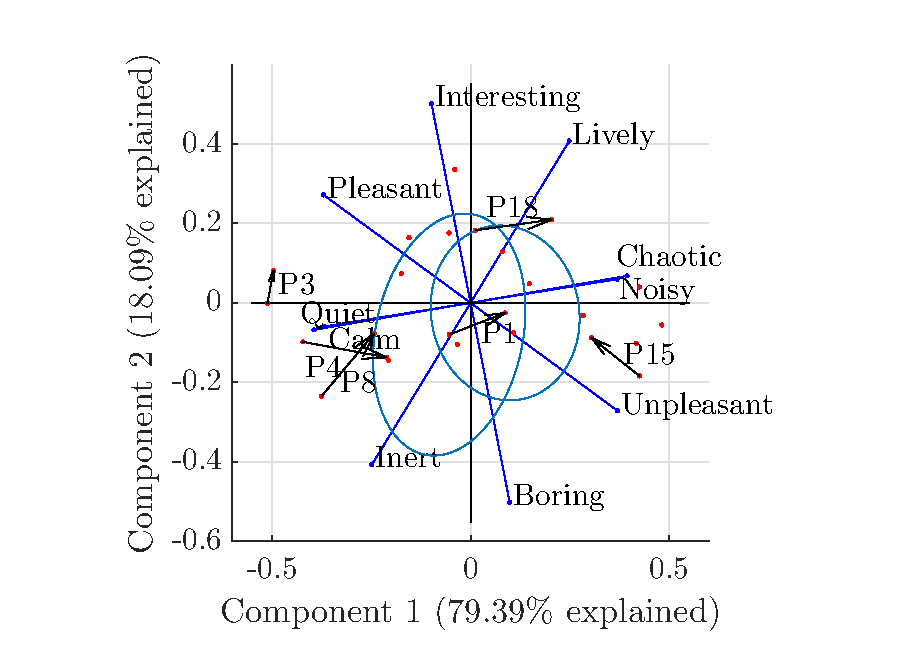
\includegraphics[width=0.8\columnwidth]{figures/pca_p1.eps}
    \caption{Biplot of the principal components analysis of average assessments for the 5 general questions on the 6 recorded and 19 replicated scenes (n=25). Arrows show discrepancies between corresponding recorded and replicated scenes. For the P1 recording location the standard deviation of the projection of individual responses is shown using ellipses.}\label{fig:pspace_rec}
\end{figure}
\begin{figure}[h]
    \centering
    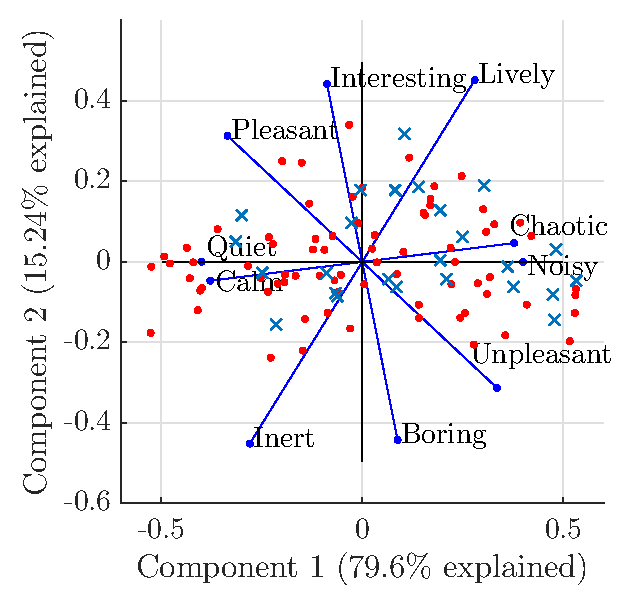
\includegraphics[width=0.8\columnwidth]{figures/pca_sim.eps}
    \caption{Biplot of the principal components analysis of average assessments for the 5 general questions on the 75 simulated scenes (n=75). Assessments of simulated scenes are projected as dots, and recorded and replicated scenes are projected as crosses.}\label{fig:pspace_sim}
\end{figure}


\subsection{Acoustical indicators for soundscape description}
\label{sec:data_inds}

Based on previous studies~\cite{aumond2017, gontier2018, ricciardi2014}, several indicators are identified that correlate well with perceptual parameters. These indicators may be used to automatically annotate sound scenes in the design of a deep learning architecture for sound source recognition.

First, indicators can be computed directly from the mixed audio, without the need for information about the composition of the scene, \textit{i.e.} source activity and level. Typically this includes indicators derived from sound level measurements. For this study the following variables are computed with a time frame of 1~s using the Matlab ITA-toolbox~\cite{itatoolbox2017}:

\begin{itemize}
\item Z-weighted $L_{eq}$ and A-weighted $LA_{eq}$ equivalent sound levels in dB and dBA respectively.
\item $L_{10}$, $L_{50}$ and $L_{90}$: 10th, 50th and 90th percentiles of the Z-weighted sound level. The $L_{10}$ is often associated to events and the $L_{90}$ to background activity, while the $L_{50}$ is a measurement of the overall sound level.
\item $LA_{50}$: 50th percentile of the A-weighted sound level, with similar properties as the $L_{50}$.
\item $L_{50, 1kHz}$: 50th percentile of the Z-weighted sound level for the 1kHz frequency band, also a good descriptor of the overall sound level of the scene.
\item $LA_{10}-LA_{90}$: Emergence indicator included in the pleasantness model presented in~\cite{ricciardi2014}.
\end{itemize}

The time and frequency second derivative ($TFSD$) is introduced in~\cite{aumond2017} as a descriptor of source activity. Its expression is:

\begin{equation}
TFSD_{f, t} = \frac{\lvert\frac{d^2L(f, t)}{dfdt}\rvert}{\sum_{f_1=31.5Hz}^{f_1=16kHz}\lvert\frac{d^2L(f_1, t)}{df_1dt}\rvert}
\end{equation}
where $L(f, t)$ is the third-octave spectrum of the signal. This indicator represents the variations in both the time and frequency dimensions to highlight sources of interest. For example, bird activity is characterized by narrow-band energy with fast paced variations in time, which translates into high $TFSD$ values in the corresponding frequency range. As a baseline indicator for source activity, the $TFSD$ is computed for the 4kHz band and 125ms measurements ($TFSD_{4kHz(1/8s)}$), and for the 500Hz band with 1s measurements ($TFSD_{500Hz, 1s}$) as estimates of the contribution of birds and voices respectively.

The simulation process of the scenes outputs ground truth source contributions as separate channels. Additional indicators are computed on the separated audio signals for the traffic, voices and birds sources: The equivalent sound level $L_{eq, s}$ for source $s$ and the source emergence $\Delta L_{s}$, taken as the difference between the equivalent sound level of source $s$ and that of all other sources combined.

Next, the $\hat T_s(\alpha, \beta)$ time of presence approximation proposed in~\cite{gontier2018} is computed. $\hat T_s(\alpha, \beta)$ is based on a binary source emergence model computed on the third-octave band emergence spectrum $\Delta L_{s}(t, f)$. It is parametrized by $\alpha$ and $\beta$ thresholds:

\begin{align}\label{eq:ts}
\hat T_s(\alpha, \beta) &= \frac{1}{N_t}\sum_{t = 1}^{N_t}\mathbbm{1}\left[ \frac{\sum_{f = 1}^{N_f}\Delta L_{s}(t, f)\mathbbm{1}_{\Delta L_{s}(t, f)>\alpha}}{\sum_{f = 1}^{N_f}\mathbbm{1}_{\Delta L_{s}(t, f)>\alpha}}>\beta \right]\\
\alpha_{opt},\beta_{opt} &= \argmax_{\alpha, \beta}\frac{1}{N_s}\sum_{s = 1}^{N_s}r\left(T_{s, p}, \hat T_s(\alpha, \beta)\right)
\end{align}

where $r$ is the Pearson's correlation coefficient, $s$ denotes the sound source, $N_s$ is the number of sources in the taxonomy and equals 3 in this study, $t$ is the time frame and $T_{s, p}$ corresponds to the perceived time of presence assessments averaged per scene. This indicator evaluates the presence or absence of a given source in a small time frame. First, frequency bands for which the source is emergent by more than the $\alpha$ threshold value are isolated. Then, the source is considered present if the emergence for these bands is on average greater than the $\beta$ threshold. A time of presence estimation is obtained for each source by averaging along the $N_t$ time frames composing the scene. The optimal threshold values are optimized once in this study on the whole perceptual experiment corpus, and found as $\alpha_{opt} = -14dB$ and $\beta_{opt} = -7dB$.

In the remainder of this paper, the subscript $s$ is replaced with the corresponding source initial: $T$ for traffic, $V$ for voices and $B$ for birds.

The considered indicators are compared to subjective assessments obtained during the listening test to identify their capacity to explain dimensions of soundscape perception. The analysis is performed using the arithmetic mean of subjective assessments over all participants for replicated and simulated scenes. The source-specific sound level $L_{eq, s}$, emergence $\Delta L_{s}$ and estimated time of presence $\hat T_s(\alpha, \beta)$ indicators cannot be directly computed on the 6 recorded scenes, as their ground truth source composition is unknown. Thus, these 6 scenes are excluded of the study. Two simulated scenes contained only one source, leading to infinite source emergences. Statistics including these scenes cannot be computed and they are thus excluded in this analysis, which as a result includes $n=92$ scenes.

Table~\ref{tab:physc} shows the Pearson's correlation coefficients between computed physical indicators and perceptual assessments. First, all global sound level indicators correlate well (r>0.9) with the perceived overall loudness. Regarding source-specific perceptual parameters, the $L_{eq, s}$ correlates consistently well with the $T_{s, p}$ of corresponding source (r=0.71). Conversely, the emergence $\Delta L_s$ fails to represent the perceived bird activity, and correlations are weak for other sources. The proposed estimates of the time of presence $\hat T_s(\alpha_{opt}, \beta_{opt})$ show strong correlations to their perceived counterparts (r>0.8), though this is expected as $\alpha_{opt}$ and $\beta_{opt}$ are optimized to this aim. They also display good source discrimination properties, as no significant correlation is found between voices and birds, and perceptual assessments of traffic were correlated with those of other sources in Table~\ref{tab:percc}. They are also better predictors than the $TFSD_{500Hz, 1s}$ and $TFSD_{4kHz, 1/8s}$ indicators for voice and bird activity in this corpus. Thus, the $\hat T_s(\alpha_{opt}, \beta_{opt})$ indicator can be used to annotate simulated sound scenes in terms of estimated perceived time of presence for the three sources.

\begin{table*}
\centering
\caption{Pearson's correlation coefficients between physical and perceptual indicators (n = 92, *: p<0.05, **: p<0.01). Non significant correlations at the 5\% threshold are noted NS.}
\label{tab:physc}
\resizebox{\textwidth}{!}{
\begin{tabular}{ c | c c c c c | c c c c }
\hline
	 & P & L & OL & I & C & $L_{T, p}$ & $T_{T, p}$ & $T_{V, p}$ & $T_{B, p}$ \\ \hline
	$LA_{eq}$ & -0.86** & 0.68** & 0.92** & -0.37** & -0.88** & 0.77** & 0.66** & NS & -0.41** \\
	$LA_{50}$ & -0.84** & 0.67** & 0.91** & -0.33** & -0.87** & 0.71** & 0.63** & NS & -0.35** \\
	$L_{eq}$ & -0.88** & 0.67** & 0.91** & -0.44** & -0.88** & 0.83** & 0.71** & NS & -0.46** \\
	$L_{10}$ & -0.87** & 0.65** & 0.90** & -0.44** & -0.86** & 0.84** & 0.71** & NS & -0.47** \\
	$L_{50}$ & -0.89** & 0.65** & 0.92** & -0.43** & -0.89** & 0.77** & 0.71** & NS & -0.44** \\
	$L_{90}$ & -0.86** & 0.68** & 0.92** & -0.39** & -0.89** & 0.71** & 0.67** & NS & -0.40** \\
	$L_{50, 1kHz}$ & -0.88** & 0.69** & 0.92** & -0.42** & -0.89** & 0.74** & 0.73** & NS & -0.50** \\
	$L_{10}-L_{90}$ & NS & NS & -0.24* & NS & -0.22* & NS & NS & NS & NS \\ \hline
	$TFSD_{500Hz, 1s}$ & NS & 0.41** & NS & 0.28** & NS & -0.24* & -0.39** & 0.74** & NS \\
	$TFSD_{4kHz, 1/8s}$ & 0.52** & -0.43** & -0.49** & 0.41** & 0.52** & -0.45** & -0.54** & NS & 0.63** \\ \hline
	$L_{eq, T}$ & -0.58** & NS & 0.46** & -0.46** & -0.42** & 0.77** & 0.71** & NS & -0.36** \\
	$L_{eq, V}$ & NS & 0.50** & 0.31** & NS & -0.37** & NS & NS & 0.71** & -0.40** \\
	$L_{eq, B}$ & 0.27* & NS & NS & 0.35** & NS & -0.25* & -0.24* & NS & 0.71** \\ \hline
	$\Delta L_T$ & -0.45** & NS & 0.26* & -0.59** & -0.22* & 0.63** & 0.66** & -0.51** & -0.26* \\
	$\Delta L_V$ & NS & 0.50** & NS & 0.35** & NS & -0.27** & -0.38** & 0.59** & NS \\
	$\Delta L_B$ & 0.21* & -0.25* & -0.26* & NS & 0.25* & -0.24* & -0.25* & NS & NS \\ \hline
	$\hat T_T(\alpha_{opt}, \beta_{opt})$ & -0.53** & NS & 0.35** & -0.57** & -0.29** & 0.56** & 0.81** & -0.39** & -0.37** \\
	$\hat T_V(\alpha_{opt}, \beta_{opt})$ & NS & 0.44** & NS & 0.35** & NS & NS & -0.39** & 0.81** & NS \\
	$\hat T_B(\alpha_{opt}, \beta_{opt})$ & 0.56** & -0.30** & -0.46** & 0.55** & 0.51** & -0.46** & -0.57** & NS & 0.91** \\ \hline
\end{tabular}
}
\end{table*}


\section{Prediction of time of presence of sources}
\label{sec:pred}

\subsection{Deep learning for presence prediction}
\label{sec:pred_deep}

A deep learning model is implemented using the Python Pytorch~\cite{paszke2017} framework and trained on the corpus presented in Section~\ref{sec:data_corp} for source time of presence prediction.

The developped model should extract relevant source information from a representation of the audio signal. Typically, spectral representations are preferred to the raw audio waveform because of the regularities they underline in the signal. Here, the third-octave spectrum is considered as it is commonly used in acoustic monitoring applications~\cite{ardouin2018, gontier2017}. Third-octave spectra are computed for 125~ms frames and 29 frequency bands in the $20~Hz - 12.5~kHz$ range as the input signal representation. Instead of a regression task where the output is directly the time of presence, a multiple label classification task on 1~s texture frames is preferred as the resulting training procedure is easier. Individual inputs are thus obtained by splitting the resulting spectrograms into texture windows of 1~s duration. The spectral blocks of dimension 29x8 are then processed independently by the model.

Ground truth target outputs are associated to each input frame to train the model. Considering the results discussed in Section~\ref{sec:data_inds}, the $\hat T_s(\alpha_{opt}, \beta_{opt})$ time of presence estimation seems well suited to automatically label the dataset for this task. Binary presence values on 1~s frames obtained during the $\hat T_s(\alpha_{opt}, \beta_{opt})$ computation before averaging in eq.\ref{eq:ts} are thus used as individual weak labels.

The architecture of the model is shown in Figure~\ref{fig:deep_arch}. The model includes 4 blocks of convolutional layers followed by leaky rectified linear unit (LeakyReLU) activations of expression $y = max(0.1x, x)$. The convolutional layers have respectively 128, 64, 32 and 32 output channels, and a common kernel size of 5x5. The output of the last block is flattened then goes through a fully connected layer with output size 3. A final sigmoid activation is used in order to obtain outputs in the 0-1 range, which correspond to the presence of traffic, voices and birds in the 1~s frame respectively. During training these values are directly compared to presence labels given by $\hat T_s(\alpha_{opt}, \beta_{opt})$ using a binary cross-entropy cost function:

\begin{equation}
BCE(y, \hat y) = -\sum_s y_s log\left(\hat y_s\right) + (1-y_s) log\left(1-\hat y_s\right)
\end{equation}
where $s$ is the source, $y_s$ and $\hat y_s$ are the target and predicted presence for source $s$ in the 0-1 range. This loss function is minimized using the Adam algorithm~\cite{kingma2015} on batches of 1~s examples. During evaluation, a threshold of 0.5 is independently applied to the 3 outputs to obtain a binary presence value for each source: each source is considered absent when the model outputs a value lower than 0.5 and present when it outputs 0.5 or higher. The time of presence estimation is then obtained by averaging presence labels of all 1~s time frames corresponding to the same scene.

\begin{figure}[h!]
    \centering
    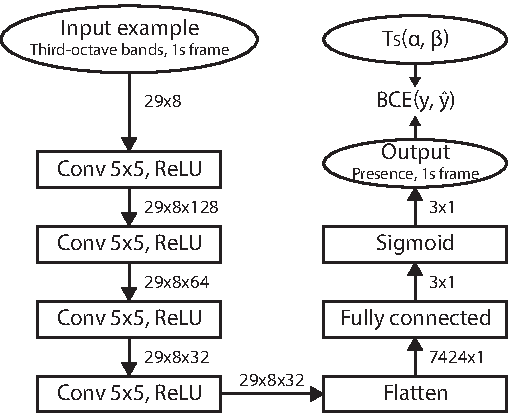
\includegraphics[width=\columnwidth]{figures/deep_arch.pdf}
    \caption{Architecture of the deep learning model used for source presence prediction.}\label{fig:deep_arch}
\end{figure}

\subsection{Results}
\label{sec:pred_res}

The performance of the source detection deep learning architecture presented in Section~\ref{sec:pred_deep} on the evaluation dataset is summarized in Table~\ref{tab:perf_cmp}. The overall presence detection accuracy is 92.11\%. The model performs similarly well for the three sources, ranging from 90.08\% for birds to 94.09\% for traffic. Regarding the type of errors, they are equally split between false positives and false negatives. Though, these rates vary depending on the type of source. Traffic has a very low false positive rate at 2.46\% and high false negative rate, while birds display the highest false positive rate at 12.30\%. This is expected given the spectral content related to these sources. Traffic is usually located in lower frequency bands than voice or bird events, but may contain high frequency components mistaken for birds by the model. The resulting error on the time of presence is 0.12 RMSE overall on a 0-1 scale, and is close for the three sources.

\begin{table*}[h!]
\centering
\caption{Performance of the model predicting source presence with binary ground truth labels obtained from $\hat T_s(\alpha_{opt}, \beta_{opt})$. Presence metrics are computed for n=8600 1s frames and time of presence metrics on n=200 45s scenes. (TP: true positive, TN: true negative, FP: false positive, FN: false negative)}
\label{tab:perf_cmp}
%\resizebox{\columnwidth}{!}{
\begin{tabular}{ c | c | c c c }
\hline
	 & All sources & Traffic & Voices & Birds \\ \hline
	Presence accuracy (\%) &  92.11 & 94.09 & 92.15 & 90.08 \\
	Presence TP (\%) & 91.96 & 92.70 & 89.93 & 93.37 \\
	Presence TN (\%) & 92.30 & 97.54 & 94.76 & 87.70 \\
	Presence FP (\%) & 7.70 & 2.46 & 5.24 & 12.30 \\
	Presence FN (\%) & 8.04 & 7.30 & 10.17 & 6.63 \\ \hline
	$\hat T_s(\alpha_{opt}, \beta_{opt})$ RMSE & 0.12 & 0.13 & 0.10 & 0.11 \\
\end{tabular}
%}
\end{table*}

\section{Application to pleasantness prediction}
\label{sec:app}

In the context of urban soundscape quality assessment, pleasantness emerges as the first affective dimension~\cite{axelsson2010}. Pleasantness has been modeled from both the perceived overall loudness in a scene~\cite{blauert1997, jekosch2004} and its content in terms of active sources~\cite{axelsson2010, lavandier2006, ricciardi2014, aumond2017}. To demonstrate the potential of the proposed method for predicting the time of presence of sources, it is applied to pleasantness estimation.

\subsection{Models of pleasantness}
\label{sec:app_mdls}

\begin{table*}[t]
\centering
\caption{Pearson's correlation coefficients between perceptual scales at the scene level (n=100, *: p<0.05, **: p<0.01)}
\label{tab:percc}
%\resizebox{\columnwidth}{!}{
\begin{tabular}{ c | c c c c c c c c c }
\hline
	 & P & L & OL & I & C & $L_{T, p}$ & $T_{T, p}$ & $T_{V, p}$ & $T_{B, p}$ \\ \hline
	P & 1 & -0.53** & -0.89** & 0.66** & 0.88** & -0.82** & -0.76** & 0.05 & 0.57** \\
	L &  & 1 & 0.76** & 0.06 & -0.78** & 0.39** & 0.17 & 0.60** & -0.36** \\
	OL &  &  & 1 & -0.39** & -0.96** & 0.71** & 0.59** & 0.17 & -0.45** \\
	I &  &  &  & 1 & 0.35** & -0.55** & -0.67** & 0.38** & 0.48** \\
	C &  &  &  &  & 1 & -0.67** & -0.55** & -0.24* & 0.48** \\
	$L_{T, p}$ &  &  &  &  &  & 1 & 0.79** & -0.15 & -0.41** \\
	$T_{T, p}$ &  &  &  &  &  &  & 1 & -0.35** & -0.42** \\
	$T_{V, p}$ &  &  &  &  &  &  &  & 1 & -0.21* \\
	$T_{B, p}$ &  &  &  &  &  &  &  &  & 1 \\ \hline
\end{tabular}
%}
\end{table*}

Baseline models of pleasantness are constructed using data from the experiment in Section~\ref{sec:data_exp}. We first study the relationships between perceptual scales with respect to existing work. Table~\ref{tab:percc} shows the Pearson's correlation coefficients between pairs of parameters with assessments averaged for each scene (n=100). The resulting values are consistent with the literature~\cite{aumond2017, gontier2018}, both for the relations to source contributions and between general scales, as discussed in Section~\ref{sec:data_val}. Indeed, pleasantness (P) is mainly influenced negatively by overall loudness (OL) and traffic and positively by birds. In previous studies a small positive contribution of voices to pleasantness was found, while no direct relation is visible from the data gathered in this study. This can be explained by the choice of speech samples used during generation, which consist of read audiobooks extracts and thus may sound unnatural in the considered urban environments. Liveliness (L) is here negatively though weakly (r=-0.36) correlated with the presence of birds, while no significant relation was found in previous studies. However, its correlation with the presence of human voices is the strongest (r=0.60), as suggested by~\cite{axelsson2010}. Relations between source-specific parameters are also weak with the exception of traffic being negatively correlated with birds (r=-0.42). The perceived sound level of passing vehicles $L_{T, p}$ is a potential alternative to the time of presence of traffic $T_{T, p}$, as it displays higher correlations with general scales and lower correlations with other source-specific parameters.

Multilinear regression models of pleasantness are built as a function of the overall loudness (OL) and source-specific parameters ($L_{T, p}$, $T_{T, p}$, $T_{V, p}$, $T_{B, p}$) with assessments averaged for each scene (n=100). All 31 combinations of the 5 predictors are considered, but to ensure that no multi-collinearity is present between predictors a variance inflation factor (VIF) test is performed prior to each regression. Only combinations for which all predictors verify $VIF<5$ are considered valid. The best resulting models in terms of $R^2_{adj}$ with statistically significant coefficient estimates ($p<0.05$) are:

\begin{align}
\begin{split}
\hat P_{1, p} & = 8.56 - 0.63~OL - 0.20~L_{T, p} + 0.11~T_{V, p}\\
&\qquad + 0.14~T_{B, p} \label{eq:pp1}
\end{split}\\
\begin{split}
\hat P_{2, p} & = 8.99 - 0.67~OL - 0.15~T_{T, p} + 0.08~T_{V, p}\\
&\qquad + 0.12~T_{B, p} \label{eq:pp2}
\end{split}
\end{align}

Because of the collinearity between $L_{T, p}$ and $T_{T, p}$, both models have very similar formal expressions, with important negative contributions of the overall loudness and traffic activity. A small positive contribution of the time of presence of voices is also found despite no significant correlation underlined in Table~\ref{tab:percc}.

Similarly, multilinear regression models of pleasantness are constructed using acoustical indicators described in Section~\ref{sec:data_inds}. Namely the $L_{50}$ and $\hat T_s(\alpha_{opt}, \beta_{opt})$ indicators are used as predictors, as they display the highest correlation values with the overall loudness and time of presence of sources respectively. Again, all combinations of the proposed physical variables are considered, and a VIF check ($VIF<5$) is performed on predictors to ensure that no multi-collinearity between predictors exists in a model. On the present corpus, the best model in terms of $R^2_{adj}$ is:

\begin{equation}
\hat P_{1, \varphi} = 16.74 - 0.18~L_{50} + 1.01~\hat T_B(\alpha_{opt}, \beta_{opt}) \label{eq:pphi}
\end{equation}

where $\varphi$ indicates a model from physical variables. Indicators related to traffic and voices activity are absent compared to the perceptual models. This is consistent with the results underlined in Table~\ref{tab:physc}: the $L_{50}$ used as a predictor is correlated to both traffic parameters $L_{T, p}$ and $T_{T, p}$ that appeared in perceptual models $\hat P_{1, p}$ (eq.\ref{eq:pp1}) and $\hat P_{2, p}$ (eq.\ref{eq:pp2}) respectively, and no strong contribution of objective variables representative of voices to pleasantness is identified in this corpus. These results can be attributed to the diversity of the studied corpus. Indeed, only traffic, voice and bird sources are present in simulated sound scenes, as a result global sound level measurements tend to be correlated with the presence of traffic in the simulation process. Quieter environments such as parks and quiet streets are less likely to have continuous traffic, while high sound levels in busy streets are always due to busy traffic. It is expected that including other sources such as construction noises and other transport-related contributions in such environments would lower the observed correlation. Additionally, the diversity of available isolated source extracts for scene simulation is rather low. Particularly, voice events are recordings of read english with low variations in speaker and consistently neutral expressiveness. These properties result in no significant correlation of indicators describing voice events to pleasantness for this corpus.

The $\hat P_{1, \varphi}$ model is compared to two baselines proposed in~\cite{ricciardi2014} and~\cite{aumond2017}, for which predictor variables are directly computed from the audio signal. Both models' coefficients are re-optimized on the studied data for a fair comparison:

\begin{align}
\hat P_{2, \varphi} &= 18.67 - 0.20~L_{50} - 0.02~(L_{10}-L_{90})\\
\begin{split}
\hat P_{3, \varphi} &= 30.18 - 0.16~L_{50, 1kHz} + 8.92~TFSD_{500Hz, 1s} \\
&\qquad + 2.99~TFSD_{4kHz, 1/8s}
\end{split}
\end{align}

Table~\ref{tab:pleasm} summarizes the performance of the two perceptual and three physical models. $\hat P_{1, p}$ and $\hat P_{2, p}$ display similar estimation errors, adjusted $R^2$ and correlation to assessed pleasantness. The performance of obtained perceptual models is about 0.6 (RMSE), which is below the average standard deviation of pleasantness assessments for this experiment: 1.77 on a 11-point scale. $\hat P_{1, \varphi}$ outperforms both $\hat P_{2, \varphi}$ and $\hat P_{3, \varphi}$, though a validation on a different corpus would be necessary to conclude on its capabilities. Compared to the models from perceptual parameters its $R^2_{adj}$ is about 9\% lower. Its RMSE is 0.83, which is also high compared to perceptual baselines, but acceptable considering the average standard deviation of pleasantness assessments of 1.77 in this study. Introducing the $L_{10}-L_{90}$ emergence in $\hat P_{2, \varphi}$ has no impact for the considered corpus, as the same overall performance metrics were obtained using only the $L_{50}$.

\begin{table}[h]
\centering
\caption{Performance of baseline models for pleasantness prediction (**: p<0.01).}
\label{tab:pleasm}
%\resizebox{\columnwidth}{!}{
\begin{tabular}{ c | c | c | c }
\hline
	 & $RMSE$ & $R^2_{adj}$ & $r$ \\ \hline
	$\hat P_{1, p}$ & 0.59 & 0.91 & 0.95** \\
	$\hat P_{2, p}$ & 0.61 & 0.90 & 0.95** \\ \hline
	$\hat P_{1, \varphi}$ & 0.83 & 0.82 & 0.91** \\
	$\hat P_{2, \varphi}$ & 0.90 & 0.79 & 0.89** \\
	$\hat P_{3, \varphi}$ & 0.91 & 0.78 & 0.89** \\ \hline
\end{tabular}
%}
\end{table}


\subsection{Prediction using deep learning}
\label{sec:app_deep}

The proposed deep learning method is applied to the perceptual experiment corpus to obtain estimations for the time of presence of traffic, voices and birds. These estimations are then applied to pleasantness estimation and compared to models presented in Section~\ref{sec:app_mdls}. To evaluate the model's robustness to the increased polyphony and source complexity of scenes in real-life scenarios, the listening test corpus is split in three parts: 1) the 6 recorded scenes which contain additional sources not present in the datasets simulated for the optimization of the deep learning model, 2) the 19 replicated scenes that also include additional sources as annotated in~\cite{gloaguen2017}, and 3) the 75 simulated scenes that are obtained from the same simulation process as both the development and evaluation dataset.

Pleasantness predictions are obtained by substituting time of presence estimates computed from the presence detection architecture's outputs to the $\hat P_{1, \varphi}$ model presented in Section~\ref{sec:app_mdls}. Thus, only the outputs corresponding to the presence of birds are used. Table~\ref{tab:pppred} presents the performance of pleasantness estimations using outputs from the deep learning architecture compared to those using ground truth $\hat T_s(\alpha_{opt}, \beta_{opt})$ labels computed with eq.~\ref{eq:ts} on separated source-specific channels. First, pleasantness estimations are equally effective using the model's predictions or the ground truth labels, with about 0.84 RMSE and 82\% of explained variance on the perceptual experiment corpus. This performance of the detection model is expected given the low errors on time of presence estimates in Table~\ref{tab:perf_cmp}. Labels from the detection model result in lower errors on the first sub-corpus containing replicated scenes with sources not seen during training. This result may indicate that the detection model generalizes well to additional sources, though a larger sample size would be required to confirm this interpretation. For the simulated subcorpus of the experiments all performance metrics are comparable. Applying the detection model on the corpus of recorded scenes for which ground truth pleasantness is available results in a RMSE of 1.09 and a decrease in $R^2_{adj}$. This is expected as these scenes are the most distant from the training corpus in terms of sources and scenarios.

\begin{table*}[t]
\centering
\caption{Pleasantness prediction quality on the perceptual experiment corpus using the source detection model compared to labels. The corpus is split in three parts: the 6 recorded scenes (Rec.), the 19 replicated scenes (Rep.), and the 75 scenes with simulated scenarios (Sim.).}
\label{tab:pppred}
%\resizebox{\columnwidth}{!}{
\begin{tabular}{ c | c c c c | c c c }
\hline
	Model & \multicolumn{4}{|c}{$P_{1, \varphi}$ with model outputs} & \multicolumn{3}{|c}{$P_{1, \varphi}$ with $\hat T_s(\alpha_{opt}, \beta_{opt})$ labels} \\ \hline
	Sub-corpus & All & Rec. & Rep. & Sim. & All & Rep. & Sim. \\ \hline
	RMSE & 0.84 & 1.09 & 0.68 & 0.85 & 0.83 & 0.72 & 0.86 \\ \hline
	r & 0.91** & 0.89** & 0.93** & 0.89** & 0.91** & 0.92** & 0.89** \\ \hline
	$R^2_{adj}$ & 0.82 & 0.73 & 0.82 & 0.80 & 0.82 & 0.79 & 0.79 \\ \hline
\end{tabular}
%}
\end{table*}

Pleasantness prediction for simulated scenes using the detection model is as effective as the best baseline model from Section~\ref{sec:app_mdls}. This indicates that detection errors found in Table~\ref{tab:perf_cmp} do not impact pleasantness prediction on average. Since the labels are extracted from a masking model approximating the perceived time of presence, they can be considered as "weak" labels. Thus, the deep learning model's predictions are in some cases considered erroneous but correlate better to perceptual assessments than the corresponding ground truth labels.

\section{Discussion}
\label{sec:discussion}

This study shows the potential of deep learning architectures in combination with corpora of simulated sound scenes for the perceptual characterization of sound environments. With the rich additional information about the source composition available for such corpora, new indicators are computed that outperform existing ones in their relation to the perceived time of presence of sources. Training a deep learning architecture on a large corpus of simulated scenes automatically annotated using these indicators then allows for the prediction of the time of presence in new recordings, where information about the contribution of each source is not available. The resulting predictions can be applied to the estimation of descriptors of soundscape perception such as the pleasantness.

Though, the performance of the trained model and its capacity to generalize to recorded data rely on several conditions. First, the perceptual characteristics of the simulated corpus should be comparable to that of typical urban environments. According to the results of the listening test presented in Section~\ref{sec:data_val}, the simulation process of sound scenes does not significantly affect the relations between abstract or content-related subjective descriptors, even with newly generated scenarios and a reduced source taxonomy. This is further demonstrated by the model of pleasantness found in Section~\ref{sec:app_mdls} from subjective annotations of source activity in this experiment. The perceptual models on the listening test corpus are similar to those found in previous studies with both \textit{in situ} questionnaires~\cite{aumond2017} and laboratory experiments using recordings~\cite{ricciardi2014}. Second, the quality of predictions is bound by that of annotations. Here, the proposed indicator does not perfectly correspond with the perceived time of presence obtained during the listening test. Furthermore, the indicator is computed using two parameters optimized on available subjective data, though it was found to be quite robust by using a cross-validation scheme during its optimization. While the quality of predictions from the model are encouraging, testing on a larger corpus is required to fully assess its generalization capabilities.

The methodology proposed in this paper can be extended to include additional sound sources provided that enough excerpts of isolated source occurrences are available. Indeed, the scene simulation process, the time of presence indicator, and the deep learning model are all independent from the considered taxonomy. Of course, the complexity of the learning process scales with the number of considered simultaneously active sources. Particularly, differentiating between sources with similar spectral shapes may yield higher error rates as the deep learning architecture relies on the identification of patterns in third octave spectra. To obtain sufficient amounts of data, data augmentation techniques can be used to diversify the training dataset by applying slight modifications to existing examples, such as filtering, pitch shifting or time stretching~\cite{salamon2017-2, lasseck2018}.

Future work will thus focus on studying the robustness of the proposed prediction scheme to a refined sound sources taxonomy as well as its application to a large scale sensor network.



\section*{Acknowledgements}
\label{sec:ack}

This research is funded by the French National Agency for Research, under the CENSE project (convention ANR-16-CE22-0012)


\bibliographystyle{unsrt}
\bibliography{refs}

\end{document}
